\documentclass{article}
\usepackage[utf8]{inputenc}
\usepackage[francais]{babel}

\author{Fabien Chéret\\Cyrille Piacibello\\Benjamin Lux}
\date{\today}
\title{Calcul de code Stencil 5 points sur une architecture hétérogène.}
\usepackage{graphicx}
\begin{document}
\maketitle

\section*{Introduction}
Le but de ce projet est d’élaborer un programme implémentant un code
stencil 5 points utilisant à la fois la carte graphique et tous les
processeurs disponibles.

La difficulté se trouve dans la non-homogénéité des ressources mises
en jeu, les processeurs ayant un fonctionnement différent de celui des
cartes graphiques.

De plus, la mémoire utilisée par ces deux unités de calcul n'est pas
la même, il sera donc nécessaire de transférer des données entre les
mémoires.

\section{Division de la matrice et traitement en simultané}
Pour des raisons de performance, les données envoyées à la carte
graphique doivent réunir certaines propriétés :
\begin{itemize}
\item l'adresse en mémoire doit être alignée sur 16 bits
\item l'adresse de début de la matrice doit être alignée sur 16 bits
\item la taille de la matrice à traiter doit être un multiple de 16
\end{itemize}
Ces propriétés sont difficiles à obtenir car notre matrice a des
bords.  Il faut donc prévoir de l'espace mémoire supplémentaire qui ne
sera pas utilisé.  Finalement, la figure \ref{matmem} indique la
représentation en mémoire de notre matrice.
\begin{figure}[!htf]
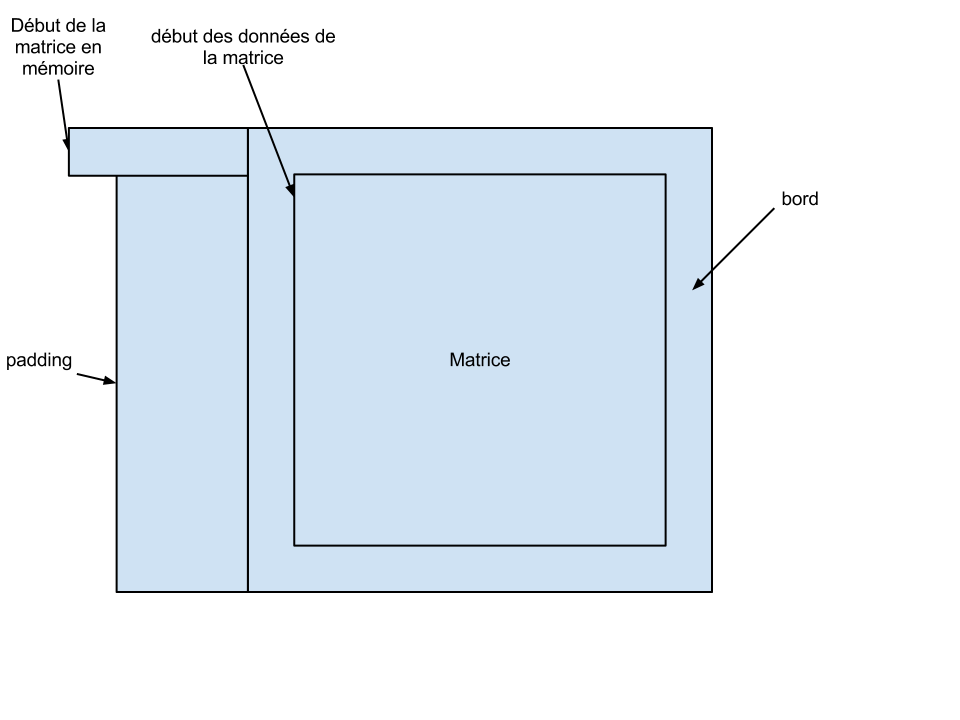
\includegraphics[scale=0.30]{matrice.png}
\caption{Représentation de la matrice en mémoire}
\label{matmem}
\end{figure}

Il y a beaucoup d'espace inutilisé, mais les performances seront
grandement améliorées.

La première étape lors de l'utilisation d'un système hétérogène a été
de séparer la matrice en deux parties afin de pouvoir la traiter
simultanément par les CPU et le GPU.

Nous avons choisi de traiter la partie haute de la matrice avec le
GPU, tandis que la partie basse sera reléguée au CPU. Cet agencement
sera efficace car la matrice et le kernel sont spécialement écrits
pour une matrice de cette forme.

Afin de lancer à la fois le traitement sur les deux unités de calcul,
nous créons un thread qui s'occupera de lancer le calcul du CPU,
tandis que le thread principal lance le traitement GPU.  De cette
manière, les deux traitements s'effectuent bien en simultané.

\section{Plusieurs itérations : transferts de données}

Le but final de ce programme est d'effectuer de nombreuses itérations
sur la matrice d'entrée.

Au niveau de l'implémentation, cela pose plusieurs problèmes :
\begin{itemize}
\item les matrices d'entrée et de sortie doivent être interverties
\item il faut récupérer les données calculées par le GPU pour que le CPU calcule les bons éléments
\item il faut récupérer les données calculées par le CPU pour que le GPU calcule les bons éléments
\end{itemize}

Pour intervertir les matrices pour le calcul CPU, il n'y a aucun
problème, il ne s'agit que d'un échange de pointeur.  Pour intervertir
les matrices données au GPU, nous avons du intégrer dans la boucle les
appels à \verb+clSetKernelArg+ qui nous a permis d'intervertir les
matrices sans avoir à les transférer de nouveau, ce qui permettra une
plus grande vitesse de traitement.


\section{Parallélisation de la partie CPU}

Pour paralléliser la partie CPU, nous avons choisi d'utiliser
\textit{OpenMP}.  La boucle de calcul se présente ainsi :
\begin{verbatim}
void stencil_multi(float* B, const float* A, int ydim)
{
for(int y=0; y<ydim; y++)
   for(int x=0; x<XDIM; x++)
     B[y*LINESIZE + x] = 0.75*A[y*LINESIZE + x] +
                         0.25*( A[y*LINESIZE + x - 1] + A[y*LINESIZE + x + 1] +
                                A[(y-1)*LINESIZE + x] + A[(y+1)*LINESIZE + x]);
}
\end{verbatim}

Il s'agit d'une double boucle for.  Nous pouvons donc paralléliser
cette boucle rapidement en ajoutant une directive \textit{OpenMP} :
\begin{verbatim}
void stencil_multi(float* B, const float* A, int ydim)
{
#pragma omp parallel for
for(int y=0; y<ydim; y++)
   for(int x=0; x<XDIM; x++)
     B[y*LINESIZE + x] = 0.75*A[y*LINESIZE + x] +
                         0.25*( A[y*LINESIZE + x - 1] + A[y*LINESIZE + x + 1] +
                                A[(y-1)*LINESIZE + x] + A[(y+1)*LINESIZE + x]);
}
\end{verbatim}
Cependant dans ce cas, seule la première boucle sera
parallélisée. Cette directive va donc créer autant de threads que de
c\oe{}urs, qui vont chacun effectuer une partie du travail total.

La solution consistant à créer N threads pour chaque coeurs n'est pas
efficace, le traitement global est ralenti à cause des changements de
contexte.

La solution finale que nous avons implémenté est donc :
\begin{verbatim}
void stencil_multi(float* B, const float* A, int ydim)
{
#pragma omp parallel for schedule(guided)
for(int y=0; y<ydim; y++)
   for(int x=0; x<XDIM; x++)
     B[y*LINESIZE + x] = 0.75*A[y*LINESIZE + x] +
                         0.25*( A[y*LINESIZE + x - 1] + A[y*LINESIZE + x + 1] +
                                A[(y-1)*LINESIZE + x] + A[(y+1)*LINESIZE + x]);
}
\end{verbatim}

L'argument \verb+schedule(guided)+ est, tests à l'appui, le plus
efficace.  Grâce à un test de plus, nous observons une accélération
d'environ 4 par rapport à la version non multi-threadée.
\section{Optimisation de la partie GPU}
Le \textit{kernel} utilisé jusqu'alors est \og naïf \fg. En effet, il
ne s'appuie que sur la mémoire globale de la carte graphique, qui est
bien plus lente que la mémoire locale, partagée dans un
multiprocesseur.  Une solution d'obtimisation serait donc de créer une
\og tuile \fg  de mémoire locale, en copiant au début du
\textit{kernel} la mémoire utile au calcul.  On espère ainsi augmenter
la vitesse du calcul, et donc du traitement global.  Cependant, la \og
tuile \fg  à copier est d'une forme assez particulière, décrite en
figure \ref{tuile}.
\begin{figure}[htp]
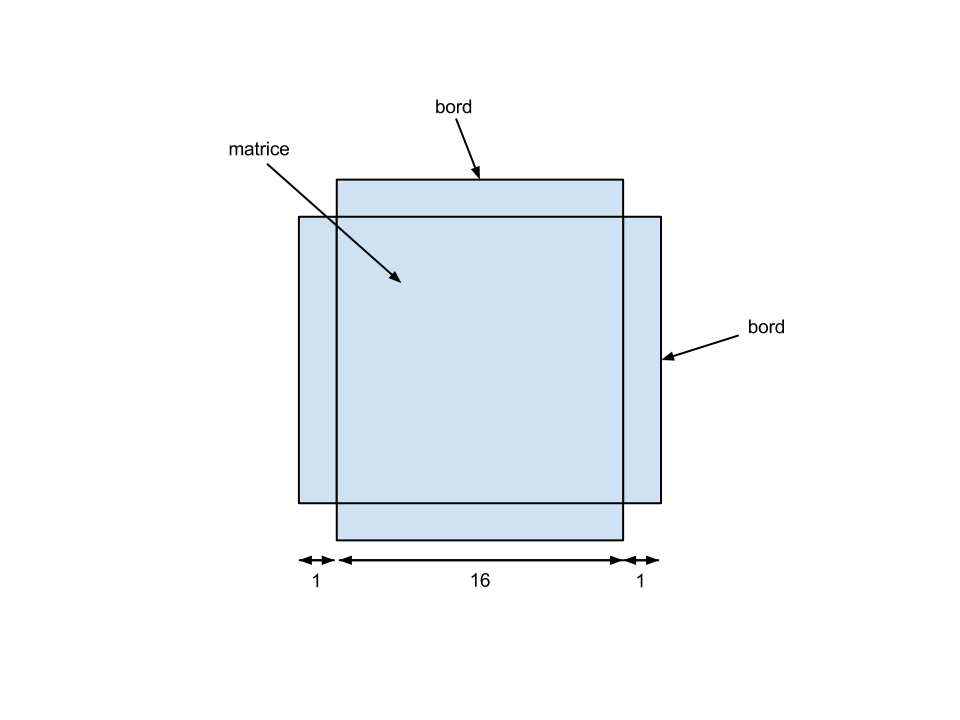
\includegraphics[scale=0.30]{/home/fabien/Projet/stencil/rapport/tuile.png}
\caption{Forme de la tuile à remplir}
\label{tuile}
\end{figure}

Lors de l'implémentation, nous nous sommes heurtés à de nombreux
problèmes. En effet, le nombre de threads nécessaire est difficile à
régler, et les indices deviennent vite compliqués à calculer.  Par
manque de temps, nous n'avons pas pu implémenter complètement cette
version optimisée, mais vous trouverez le code temporaire dans les
annexes de ce rapport en \ref{kernel}.  De plus l'abscence de
débogueur pour le code OpenCL n'a pas facilité l'implémentation ; un
outil du type \textit{gdb} aurait été fort apréciable, et il ne fait
aucun doute qu'avec cet outil, nous serions arrivé à une solution plus
facilement.

\section{Solution finale et résultats}
\subsection{Performance}
A des fins de tests, nous augmentons la taille du problème jusqu'à une
matrice de $8192\times4096$.

Afin de tester finement l'accélération du programme, nous créons un
script shell simple (voir annexe \ref{script}) qui lance le programme
en modifiant les paramètres de façon à ce que la taille de la matrice
gérée par le CPU augmente de 64 lignes à chaque itération.

\begin{figure}[htp]
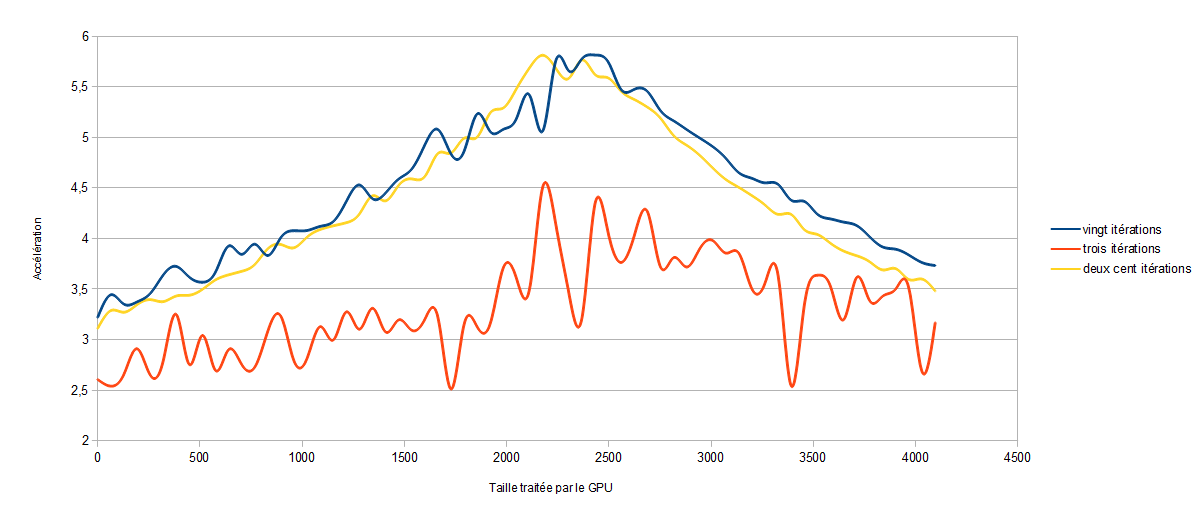
\includegraphics[scale=0.30]{/home/fabien/Projet/stencil/rapport/acceleration.png}
\caption{Accélération en fonction de la taille et du nombre d'itérations}
\label{acceleration}
\end{figure}

Ces données sont utiles, car elles permettent de voir quelle est la
meilleure taille à utiliser pour que le calcul soit le plus efficace
possible.

Ici, nous pouvons donc déduire que la meilleure taille à utiliser se
situe vers $2240$ lignes pour le GPU.

Nous pouvons aussi voir que notre travail a porté ses fruits,
puisqu'on obtient une accélération supérieure à celle observée par la
version CPU multi-threadée.

\subsection{Conclusion}
Pour conclure, nous pouvons dire que notre programme est un succès,
car il présente une accélération non négligeable d'environ 6.
Cependant, ce résultat est limité par la présence de code séquentiel
(interversion des matrices, calcul du temps passé en traitement), mais
aussi par la lenteur des écritures mémoire. En effet, le transfert des
lignes, même s'il est réduit au maximum, est toujours très long.

Pour améliorer tout de même ces résultats, si nous avions plus de
temps, nous aurions fini d'implémenter le kernel optimisé utilisant la
mémoire locale de la carte graphique, ce qui aurait, on l'espère, eu
une conséquence notable sur l'accélération.

\clearpage
\section*{Annexe}
\subsection{Kernel optimisé non finalisé}
\label{kernel}
\begin{verbatim}
__kernel void
stencil(__global float *B,
        __global float *A,
        unsigned int line_size)
{

    __local float tile[18][18];

    const unsigned int x = get_global_id(0);
    const unsigned int y = get_global_id(1);

    const unsigned int xloc = get_local_id(0);
    const unsigned int yloc = get_local_id(1);

    A += line_size + 16;
    B += line_size + 16;

    for(int i=0; i<4; i++)
    {
        tile[xloc+1][yloc*4+i+1] = A[(y*4+i)*line_size + x];
    }

    const int cbx = xloc;
    const int cby = (yloc & 1) ? -1 : 16;
    const int bx = (yloc & 2) ? cbx : cby;
    const int by = (yloc & 2) ? cby : cbx;


    tile[cbx][cby+1] = A[(y*4-yloc+cby)*line_size + x];
    for(int i=0; i<4; i++)
    {
        tile[bx+1][by+1+i] = A[(y*4+i-yloc+by)*line_size + x - xloc + bx];
    }
    barrier(CLK_LOCAL_MEM_FENCE);

    for(int k=0; k<4; k++)
        B[(k + y*4)*line_size + x] = 0.75 * tile[xloc+1][yloc*4+k+1] +
                                       0.25*( tile[xloc][yloc*4+k+1] +
                                              tile[xloc+2][yloc*4+k+1] +
                                              tile[xloc+1][yloc*4+k] +
                                              tile[xloc+1][yloc*4+k+2]);


}
\end{verbatim}

\subsection{script utilisé lors des tests}
\label{script}
\begin{verbatim}
#!/bin/bash
taille=4096
i=0
str=""
while((i<taille))
do
str=$i"\t"
str=$str$(./stencil 200 $i)
echo -e $str >> sortie.txt
((i+=64))
done
\end{verbatim}
\end{document}
